% == HEATMAP MATRIX == 
\begin{figure}[ht]
    \begin{subfigure}[b]{0.49\textwidth}
        \centering{
            \resizebox{\textwidth*\real{\heatmap}}{\textwidth*\real{\heatmap} * \real{1}}{% This file was created by tikzplotlib v0.9.4.
\begin{tikzpicture}

\begin{axis}[
tick align=outside,
tick pos=left,
title={coo},
x grid style={white!69.0196078431373!black},
xmin=0, xmax=58,
xtick style={color=black},
y grid style={white!69.0196078431373!black},
ymin=0, ymax=58,
ytick style={color=black}
]
\addplot graphics [includegraphics cmd=\pgfimage,xmin=0, xmax=58, ymin=0, ymax=58] {coo-001.png};
\end{axis}

\end{tikzpicture}
}
            \caption{$W_{\text{co-cites}}$}
            \label{subfig:adj_sparse}
        }
    \end{subfigure}
    % \hfill
    % \pgfdeclareverticalshading{colormap}{0.2cm}{rgb(0.0pt)=(0,1,1); rgb(6cm)=(0.8784,0.6902,0.99998)}
    % \pgfuseshading{colormap}
    \hfill
    \begin{subfigure}[b]{0.49\textwidth}
        \centering{
            \resizebox{\textwidth*\real{\heatmap}}{\textwidth*\real{\heatmap} * \real{1}}{% This file was created by tikzplotlib v0.9.4.
\begin{tikzpicture}

\begin{axis}[
hide x axis,
hide y axis,
tick align=outside,
tick pos=left,
x grid style={white!69.0196078431373!black},
xmin=0, xmax=80,
xtick style={color=black},
y grid style={white!69.0196078431373!black},
ymin=0, ymax=80,
ytick style={color=black}
]
\addplot graphics [includegraphics cmd=\pgfimage,xmin=0, xmax=80, ymin=0, ymax=80] {coo_dense-002.png};
\end{axis}

\end{tikzpicture}
}
            \caption{$W_{\text{text}}$}
            \label{subfig:adj_dense}
        }
    \end{subfigure}
    \label{fig:sparse_dense}
    \vfill
    \centering{
        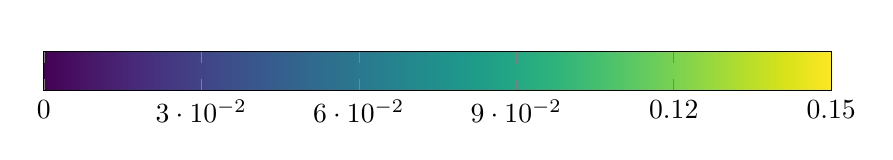
\begin{tikzpicture}
    \begin{axis}[
            hide axis,
            scale only axis,
            height=0pt,
            width=0pt,
            colormap/viridis,
            colorbar horizontal,
            point meta min=0,
            point meta max=0.15,
            colorbar style={
                    width=10cm,
                    height=0.5cm,
                    xtick={0,0.03,0.06,0.09,0.12,0.15}
                }]
        \addplot [draw=none] coordinates {(0,0)};
    \end{axis}
\end{tikzpicture}
    }
    \caption{\textbf{Heatmap of Two Different Edge Weight Matrices}}
    \label{fig:heatmap:edgeweights:compare}
\end{figure}

